

\section{Evaluation}
\label{sec:eval}

%There are two goals of this sections 1) evaluate the performance of RA primitive operations Union and Join  2) evaluate the performance of transitive closure, which is a fixed point iteration algorithm.
The goal of this section is to evaluate the performance of parallel join, parallel union and parallel transitive closure at scale.
To this end, we individually study the computation and communication components of the RA operations.
Computation is dominated by insertion of tuples and the major challenge faced is that of deduplication.
We first study the efficacy of our btree-based relation container for inserts specifically in the context of deduplication.
All our RA operations involve an all to communication phase, hence, we perform a detailed MPI all to all benchmark.
Following these two experiments, we then benchmark the efficacy of parallel union, parallel join and parallel transitive closure over a wider range of graphs.
%We first study how our data structure performs, and how well are the all to all communication primitives are supported by super computers. More specifically, we study how fast can we insert into our btree based relation class, and how efficiently can it support the task of de-duplication. This is mostly studying the computation aspect of our algorithms. Next, with the all to all tests, we benchmark the communication aspect of our algorithms.


%Radix-hash join and merge-sort join are two of the most popularly used parallel implementations of the inner join operation. Both these algorithms involve partitioning the input data so that they can be efficiently distributed to the participating processes. For example, in the radix-hash approach a tuple is assigned to a process based on the hash output of the column-value on which the join operation is keyed. With this approach, tuples on both relations that share the same hash value are always assigned to the same process. For every tuple in the left-hand side of the join relation is matched against all the tuples of the right-hand side of the join relation. Fast lookup data-structures like hash tables, or radix-trees (TRIE) can be used to organize the tuples within every process. The initial distribution of data using hashing reduces the overall computation overhead by a factor of the number of processes (n).

%More recently (Barthels et al. 2015, 2017), there has been a concerted effort to implement JOIN operations on clusters using an MPI backend. The commonly used radix-hash join and merge-sort join have been re-designed for this purpose. Both these algorithms involve a hash-based partitioning of data so that they are be efficiently distributed to the participating processes and are designed such that inter-process communication is minimized. In both of these implementations one-sided communication is used for transferring data between process. With one-sided communication the initiator of a data transfer request can directly access parts of the remote memory and has full control where the data will be placed. Read and write operations are executed without any involvement of the target machine. This approach of data transfer involves minimal synchronization between particiapting processes and have been shown to scale better that traditional two-sided communication. The implementation of parallel join has shown promising performance numbers; for example, the parallel join algorithm of (Barthels et al. 2017) ran successfully at 4,096 processor cores with up to 4.8 terabytes of input data


\subsection{Dataset and HPC platforms}
\label{sec:datasets}
We have performed our experiments using open sourced graphs available at ~\cite{}.
The graphs represent a wide range in terms of the number of edges. The last three graphs are the largest available graphs.
Transitive closure of a graph with n edges can compute upto n^2 edges for a fully connected graph. The number of edges in the transitive closure of a graph depends on the connectivity of the input graph. We found our third graph with X edges to be highly connected; the transitive closure of the graph genertaed 260 billion edges, which is 3 terabytes in size.
-- wide range in terms of number of edges
-- The transitive closure of third graph generated 260 billion edges, which corresponds to 4 tera bytes of data.

\begin{table}[]
	\begin{tabular}{lllll}
		\begin{tabular}[c]{@{}l@{}}Input graph \\ edge count\end{tabular} & Union & Join & \begin{tabular}[c]{@{}l@{}}Transitive \\ Closure\end{tabular} & Graph name \\
		412148                                                            & \checkmark      & \checkmark     &                                                               &            \\
		2100225                                                           &       &      &                                                               &            \\
		6291408                                                           &       &      &                                                               &            \\
		59062957                                                          &       &      &                                                               &            \\
		136024430                                                         &       &      &                                                               &            \\
		180292586                                                         &       &      &                                                               &            \\
		240023949                                                         &       &      &                                                               &           
	\end{tabular}
\end{table}


The experiments presented in this work were performed on
Theta at the Argonne Leadership Computing Facility
(ALCF). Theta is a Cray XC30 with a peak
performance of X petaflops, 124, 608 compute cores, 332
TiB of RAM, and 7.5 PiB of online disk storage. We used
Edison Lustre file system (168 GiB/s, 24 I/O servers and 4
Object Storage Targets). 

%Default striping was used with the Lustre file system. Mira system contains 48 racks and 768K cores, and has a theoretical peak performance of 10 petaflops. Each node has 16 cores, with 16 GB of RAM per node. I/O and interprocessor communication travels on a 5D torus network. Every 128 compute nodes has two 2 GB/s bandwidth links to two different I/O nodes, making 4 GB/s bandwidth for I/O at most. I/O nodes are connected to file servers through QDR IB. Mira uses a GPFS file system with 24 PB of capacity and 240 GB/s bandwidth.


\begin{figure*}[t]
	{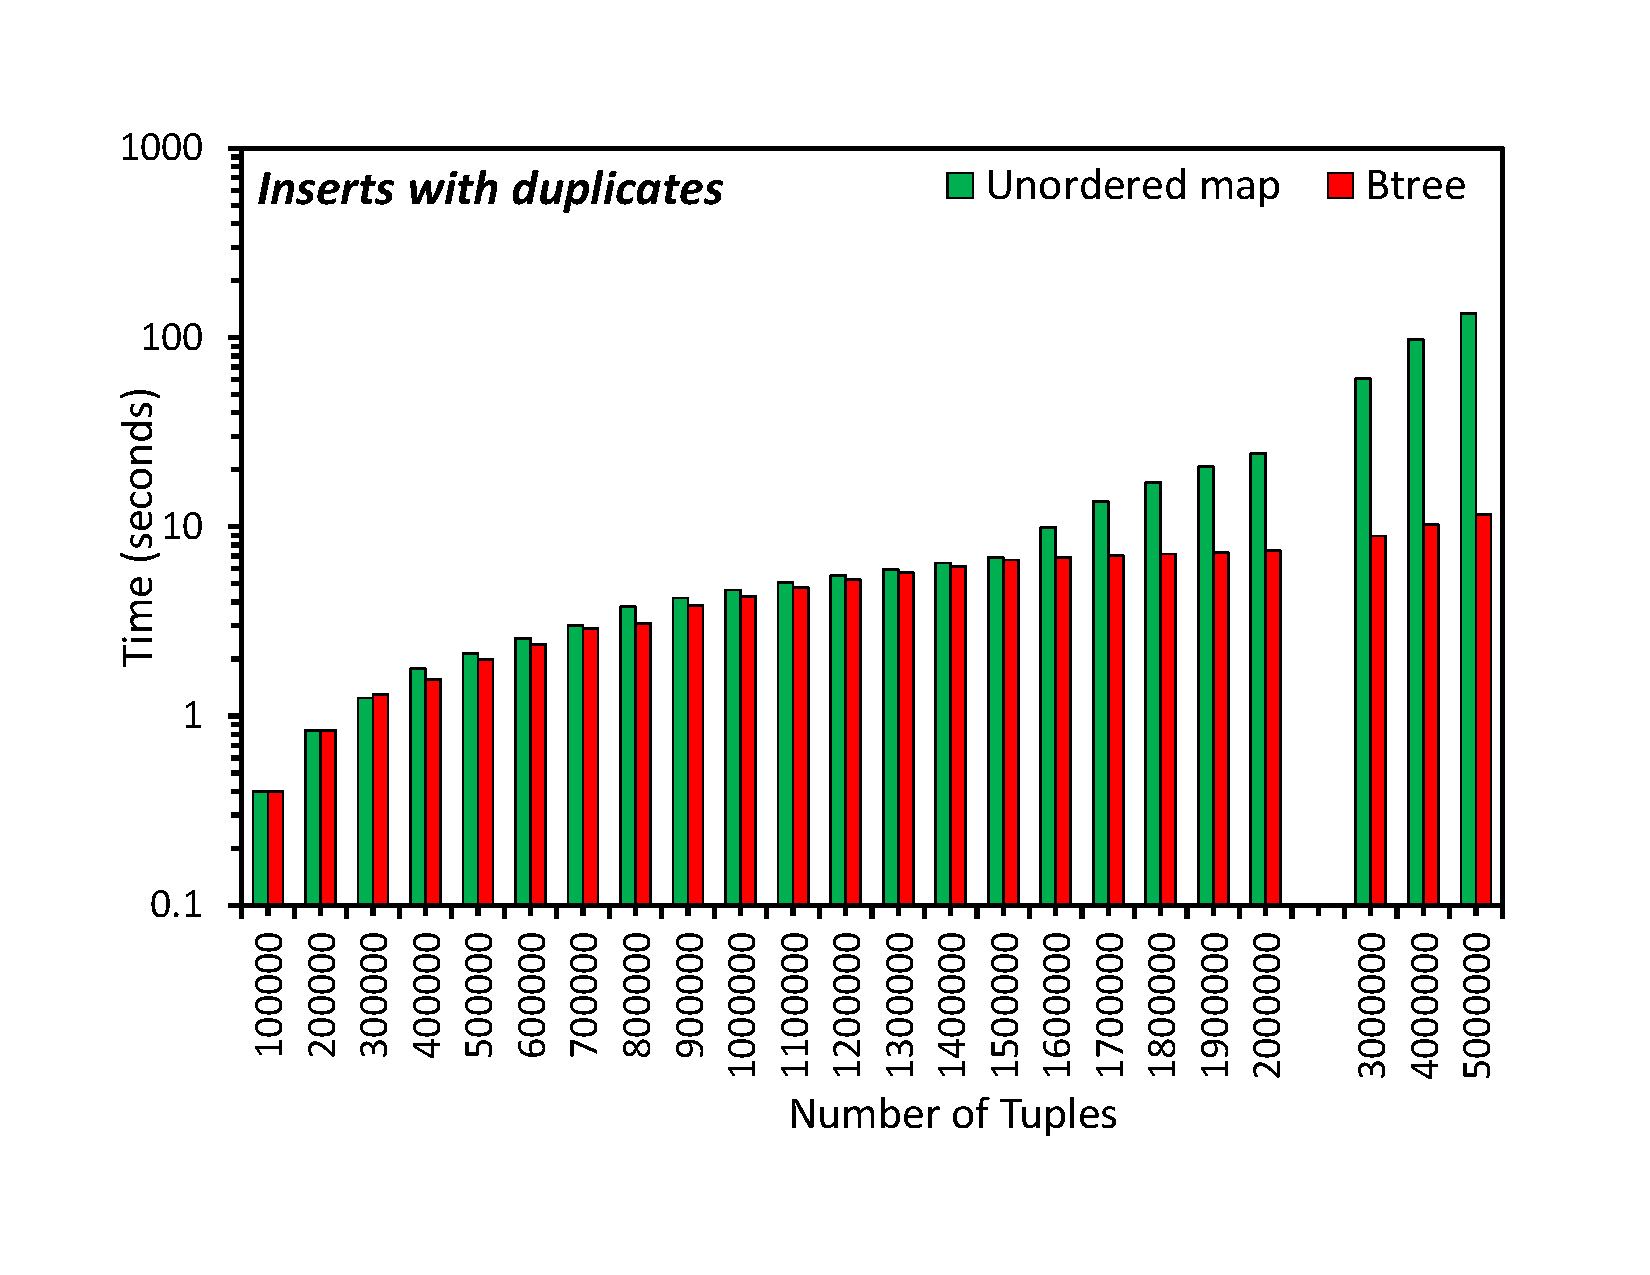
\includegraphics[width=.50\textwidth,  trim={0cm 0cm 0cm 0cm, 
			clip}]{results/inserts_with_duplicates.pdf}}\hfill%
	{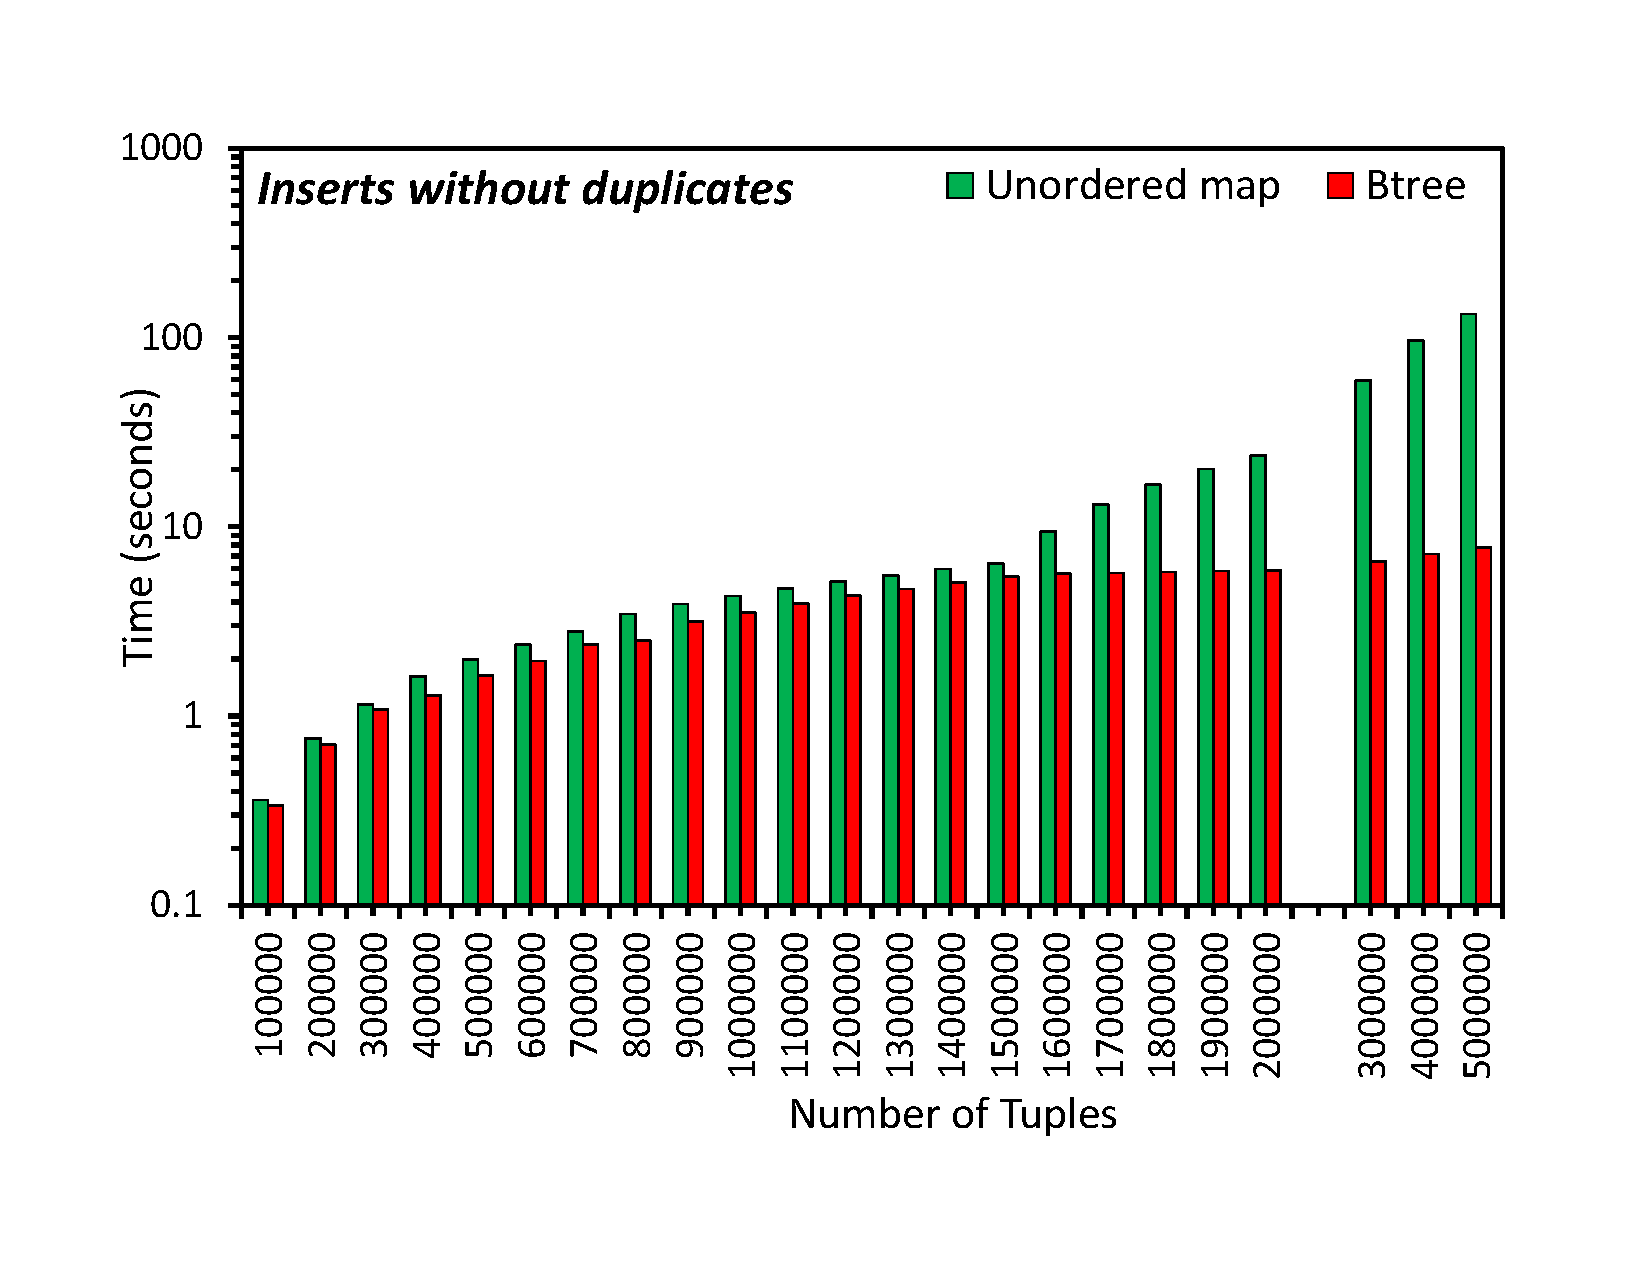
\includegraphics[width=.50\textwidth,  trim={0cm 0cm 0cm 0cm,
			clip}]{results/inserts_with_no_duplicates.pdf}}\hfill%
	\centering
	\caption{Performance evaluation of relation class implemented with btree and unordered map. (left) All tuples are distinct, (right) There are four copies of every tuple being inserted. Relation implemented with btree out-performs the unordered-map implementation.}
	\label{fig:tuple_inserts}
\end{figure*}


\subsection{Relation}
\label{sec:relation}
-- Perform two benchmarks: insertion of tuples without any duplicate and insertion of tupes each with four duplicates.
-- Relation class implemented with btrees outperforms relation with hashes.
-- btree-relation scales with increase tuple count as opposed to hash based relation that fails to scale for large number of tuples.
-- For example hash based relation takes X seconds to insert Y tuples as opposed to only Z seconds taken by btree based relation.



\begin{figure*}[t]
	{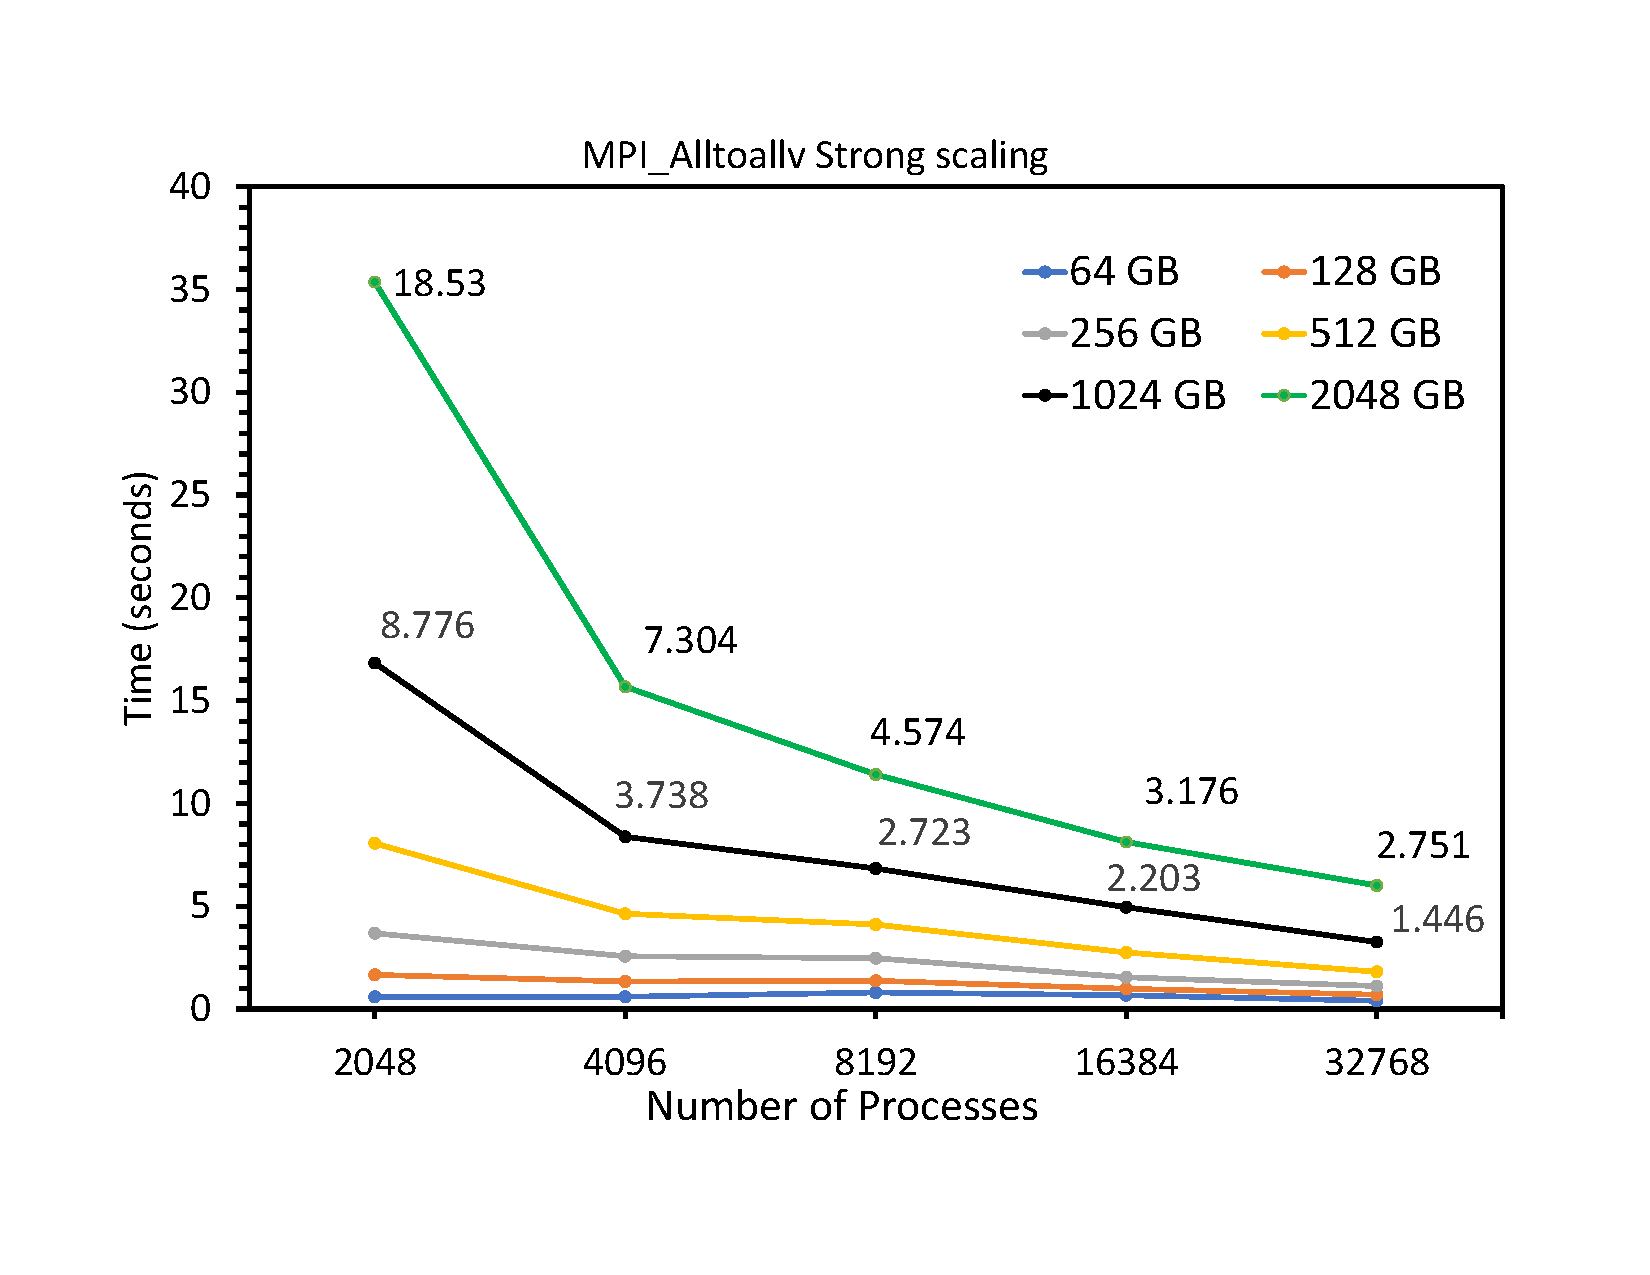
\includegraphics[width=.50\textwidth,  trim={0cm 0cm 0cm 0cm, 
			clip}]{results/all_to_all_strong.pdf}}\hfill%
	{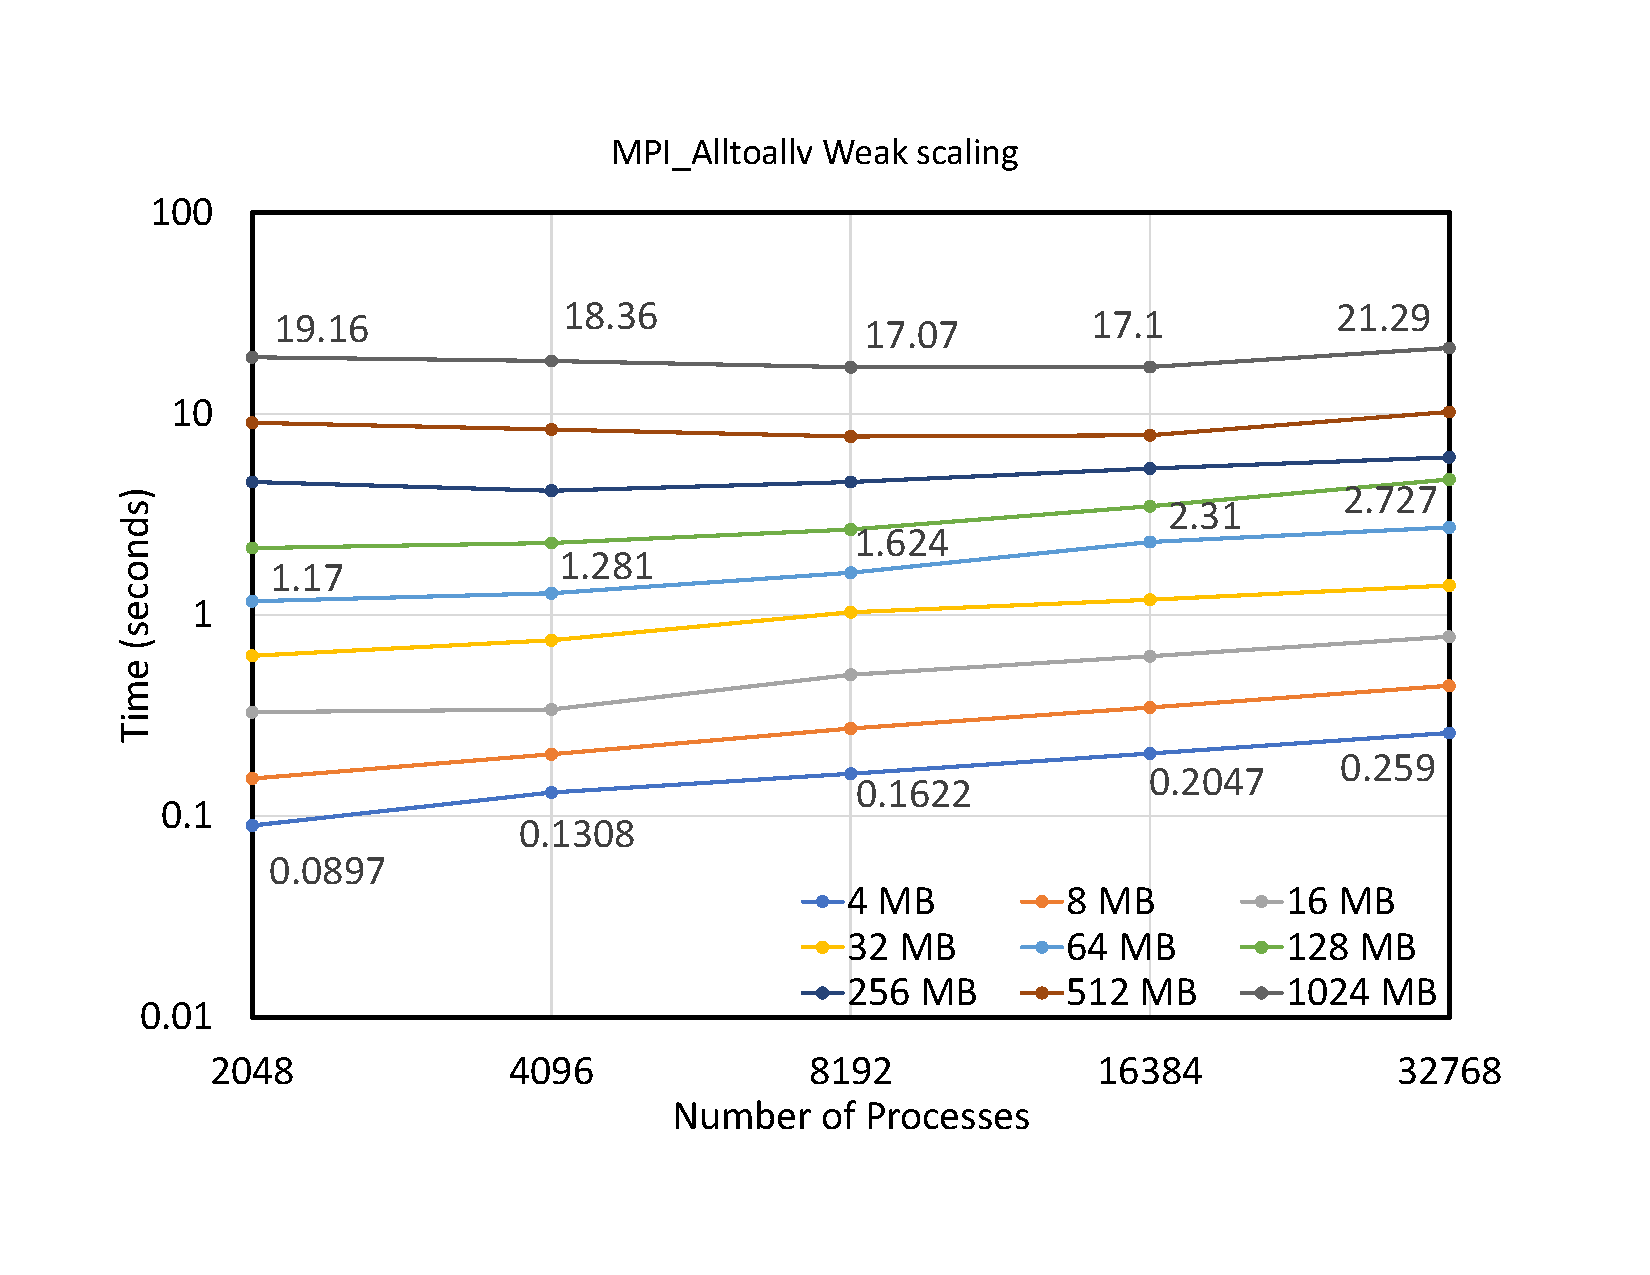
\includegraphics[width=.50\textwidth,  trim={0cm 0cm 0cm 0cm,
			clip}]{results/all_to_all_weak.pdf}}\hfill%
	\centering
	\caption{Strong (left) and Weak (right) scaling evaluation of MPI\_alltoallv function of MPI.}
	\label{fig:all_to_all}
\end{figure*}


\subsection{MPI\_All\_to\_Allv}
\label{sec:all_to_all}

-- perform both weak and strong scaling
-- configuration
-- weak scaling with accuracy X percent accuracy for per process load of Y versus Z percent accuracy for per process load of M.
-- Exhibit poor weak scaling for small load, as opposed to good weak scaling with larger volume of data.
-- X percent accuracy with strong scaling of X load. This corresponds to Y number of tuples.
-- Overall very good indication as all to all scales well, aggregate accuracy
-- different graphs would work better at different scales.

\subsection{Parallel Union}
\label{sec:union}
-- union of 7 graphs from table
-- union comprises of an io phase followed by communication and then followed by inserts
-- We compare two union types, one is where we perform io, comm and compute separates, the other is where we first perform io for all and then we bundle all our comm and then we have one phase of compute
-- scales well upto X cores., this is strong scaling.
-- faces work load deprecation at low core counts, needs more tuples for union to scale at high core counts
-- overall a good sign


\subsection{Parallel Join}
\label{sec:join}
-- setup, join of two of the largest graph, produces X number of tuples in output.
-- similar to union join scales well upto X cores, after that there is shortage of work and we do not see proper scaling.
-- communication stops to scale after X core counts. This is because there is lack of work.
-- 


\subsection{Transitive closure}
\label{sec:tc}

Computing the transitive closure of a graph involves repeated join operations until a fixed point is reached. We
use the previously discussed radix-hash join algorithm to distribute the tuples across all processes. The algorithm
can then be roughly divided into four phases: 1) Join 2) network communication 3) insertion 4) checking for a
fixed point. In our join phase every process concurrently computes the join output of the local tuples. In the next
phase every process sends the join output results to the relevant processes. This is a all-to-all communication
phase, which we implemet using MPI’s all to all routines. The next step involves inserting the join output result
received from the network to the output graph’s local partition. In the final step we check if the size of the
output graph changed on any process, if it does then we have not yet reached a fixed point and we continue to
another iteration of these 4 steps.
We performed a set of strong-scaling experiments to compute the transitive closure of graph with 412148
edges—the largest graph in the U. Florida Sparse Matrix set (Davis and Hu 2011). We used the Quartz supercomputer
at the Lawrence Livermore National Laboratory (LLNL). For our runs, we varied the number of processes
from 64 to 2048. A fixed point was attained after 2933 iterations, with the resulting graph containing 1676697415
edges. As can be seen in Figure 1, our approach takes 462 seconds at 64 cores and 235 seconds at 2048 cores, corresponds
to an overall efficiency of 6.25%. We investigated these timings further by plotting the timing breakdown
of by the four major components (join, network communication, join, fixed-point check) of the algorithm. We
observe (see Figure 2) that for all our runs the total time is dominated by computation rather than communication;
insert and join together tended to take up close to 90% of the total time. This is quite an encouraging result
as it shows that we are not bound primarily by the network bandwidth (at these scales and likely moderately
higher ones) and it gives us the opportunity to optimize the computation phase

\begin{figure*}[t]
	{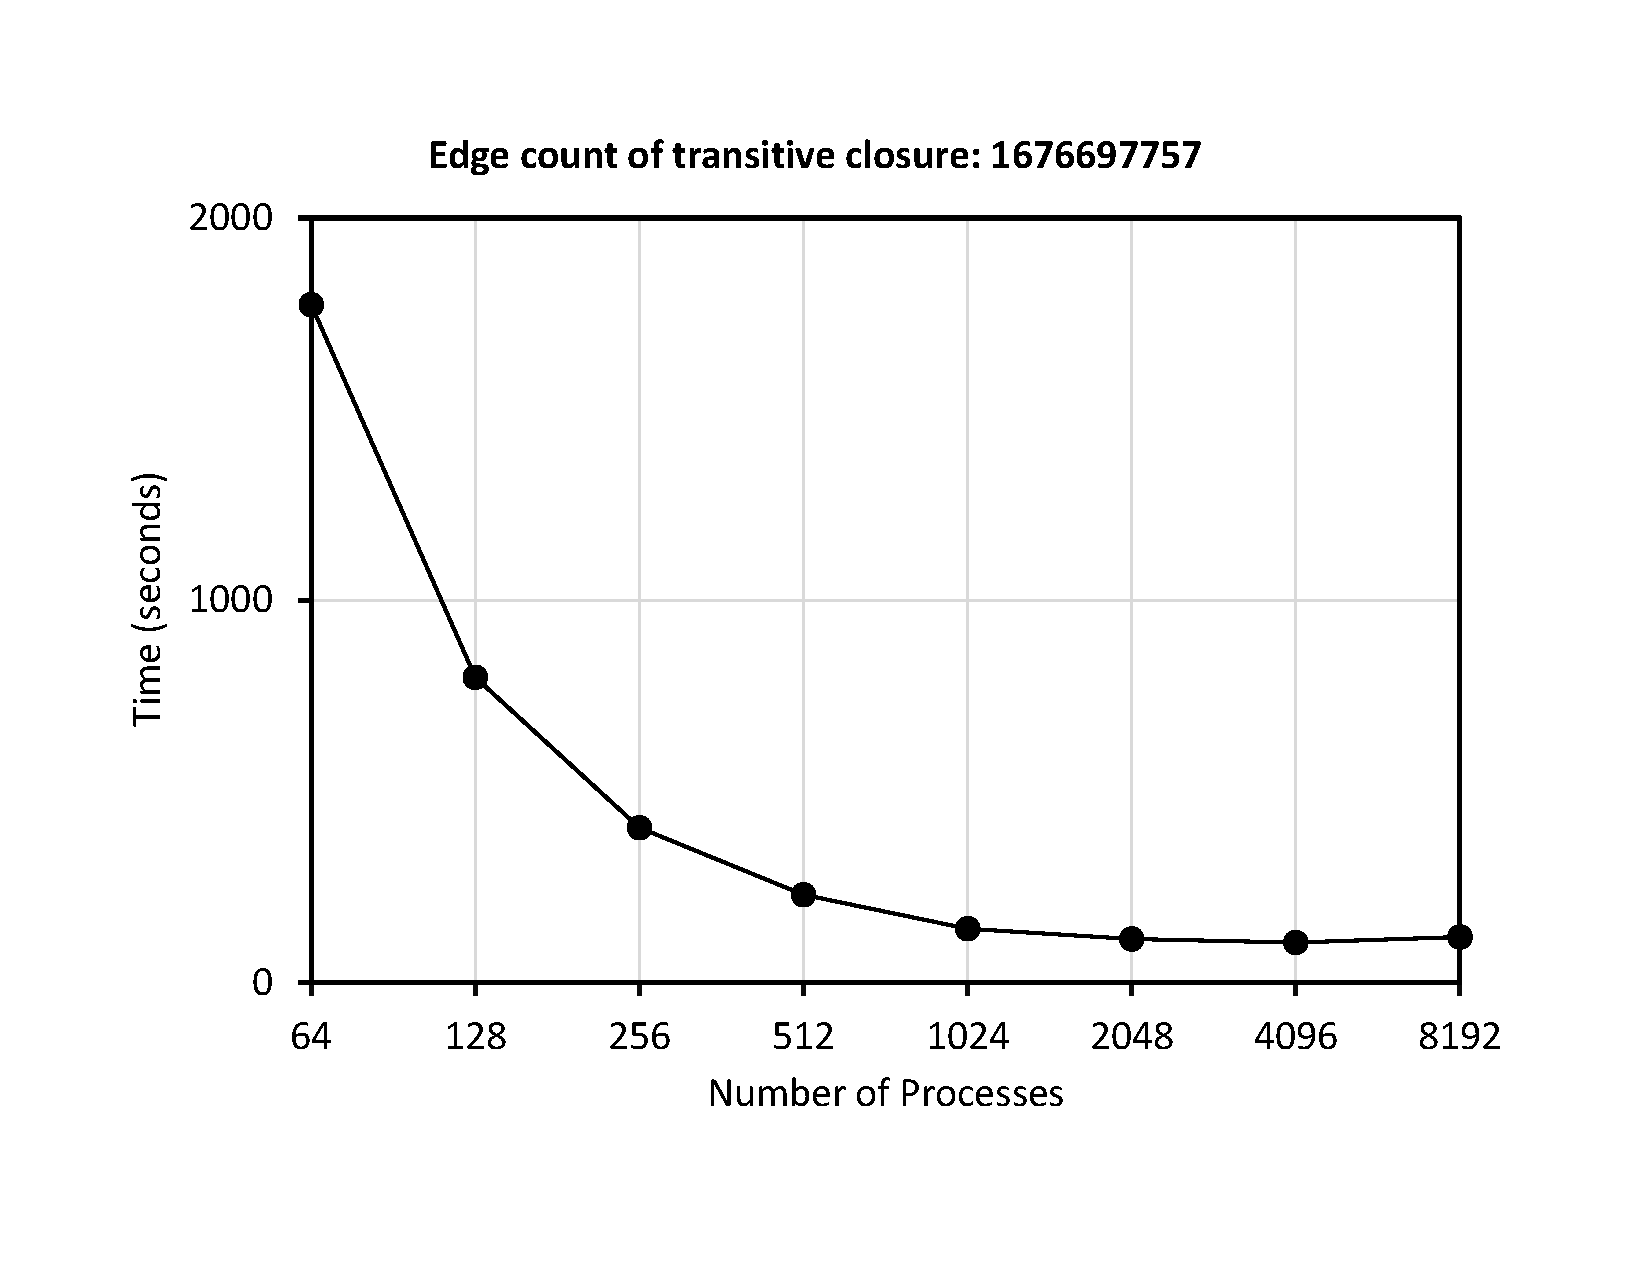
\includegraphics[width=.50\textwidth,  trim={0cm 0cm 0cm 0cm, 
			clip}]{results/TC_1_6Billion.pdf}}\hfill%
	{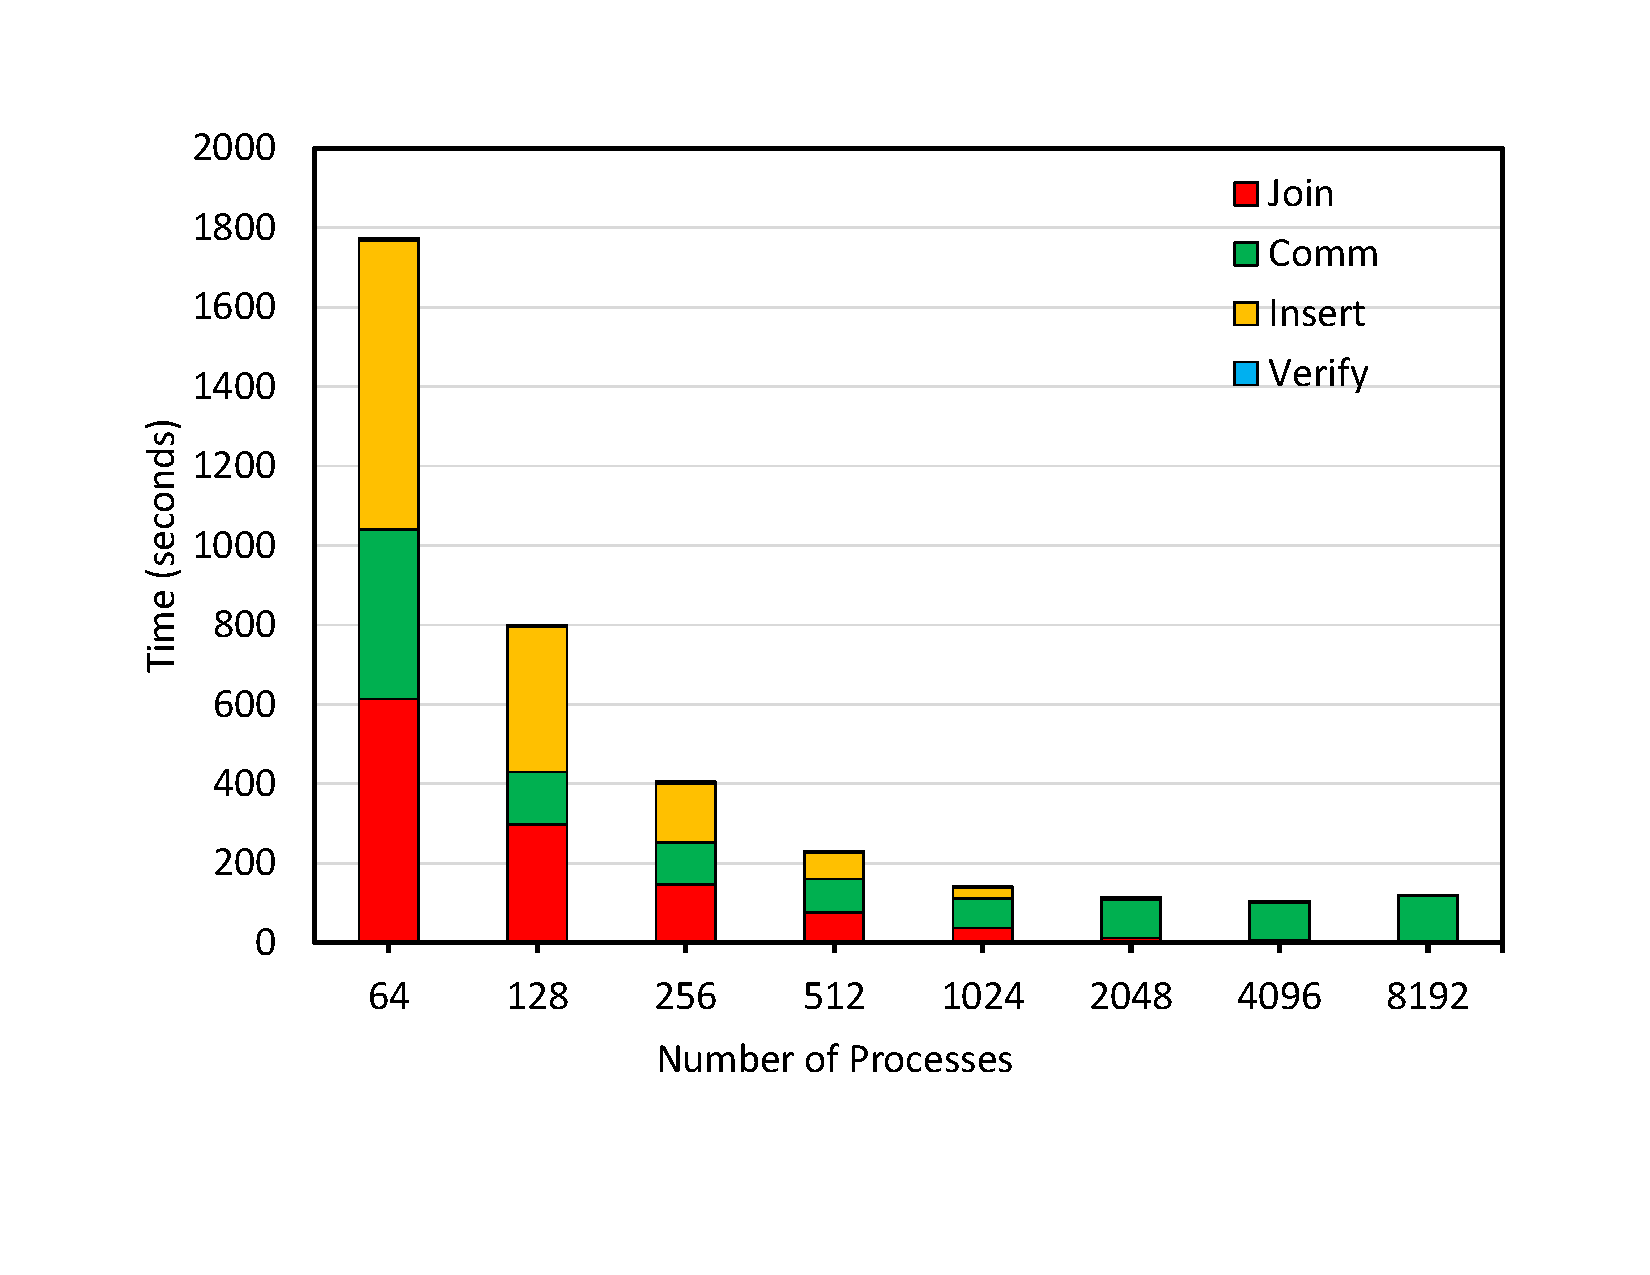
\includegraphics[width=.50\textwidth,  trim={0cm 0cm 0cm 0cm,
			clip}]{results/TC_1_6Billion_breakdown.pdf}}\hfill%
	\centering
	\caption{Transitive closure of a graph with X edges.}
	\label{fig:tc_small}
\end{figure*}


\begin{figure*}[t]
	{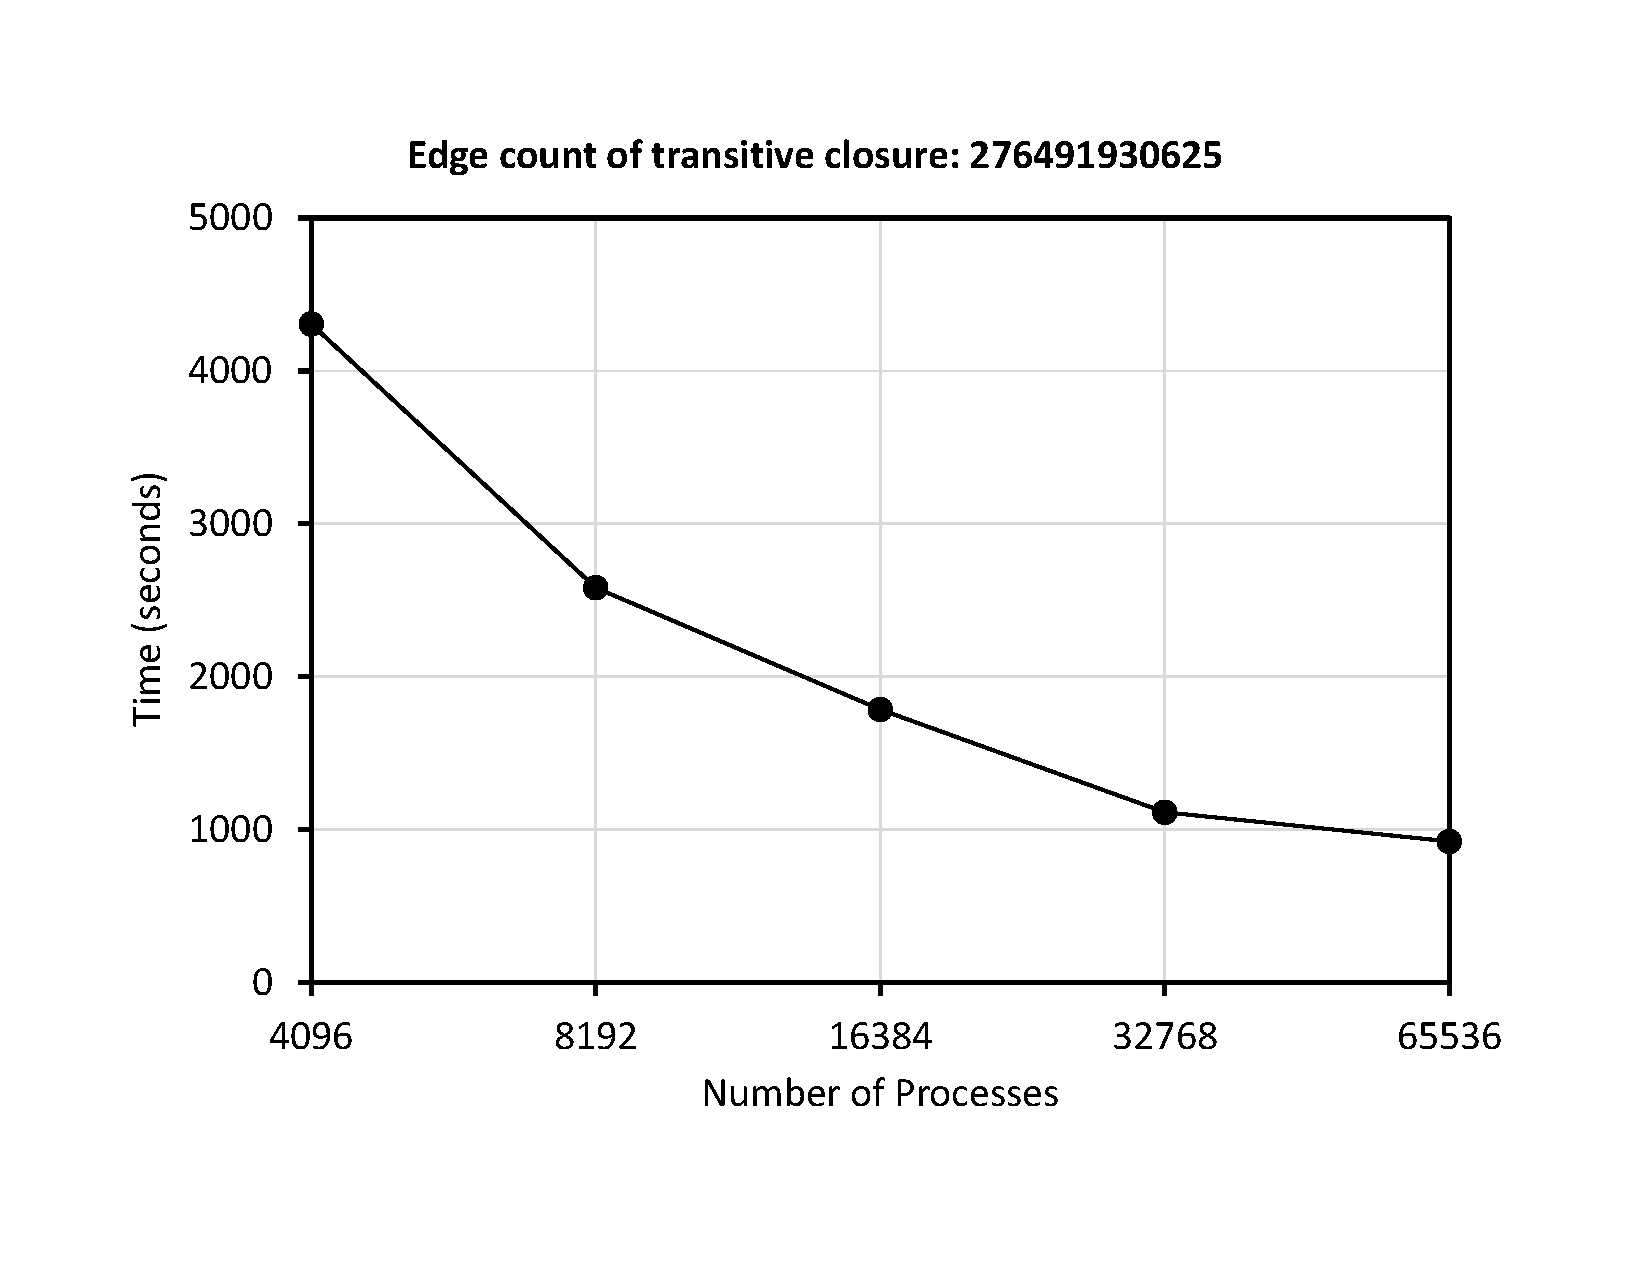
\includegraphics[width=.50\textwidth,  trim={0cm 0cm 0cm 0cm, 
			clip}]{results/TC_260Billion.pdf}}\hfill%
	{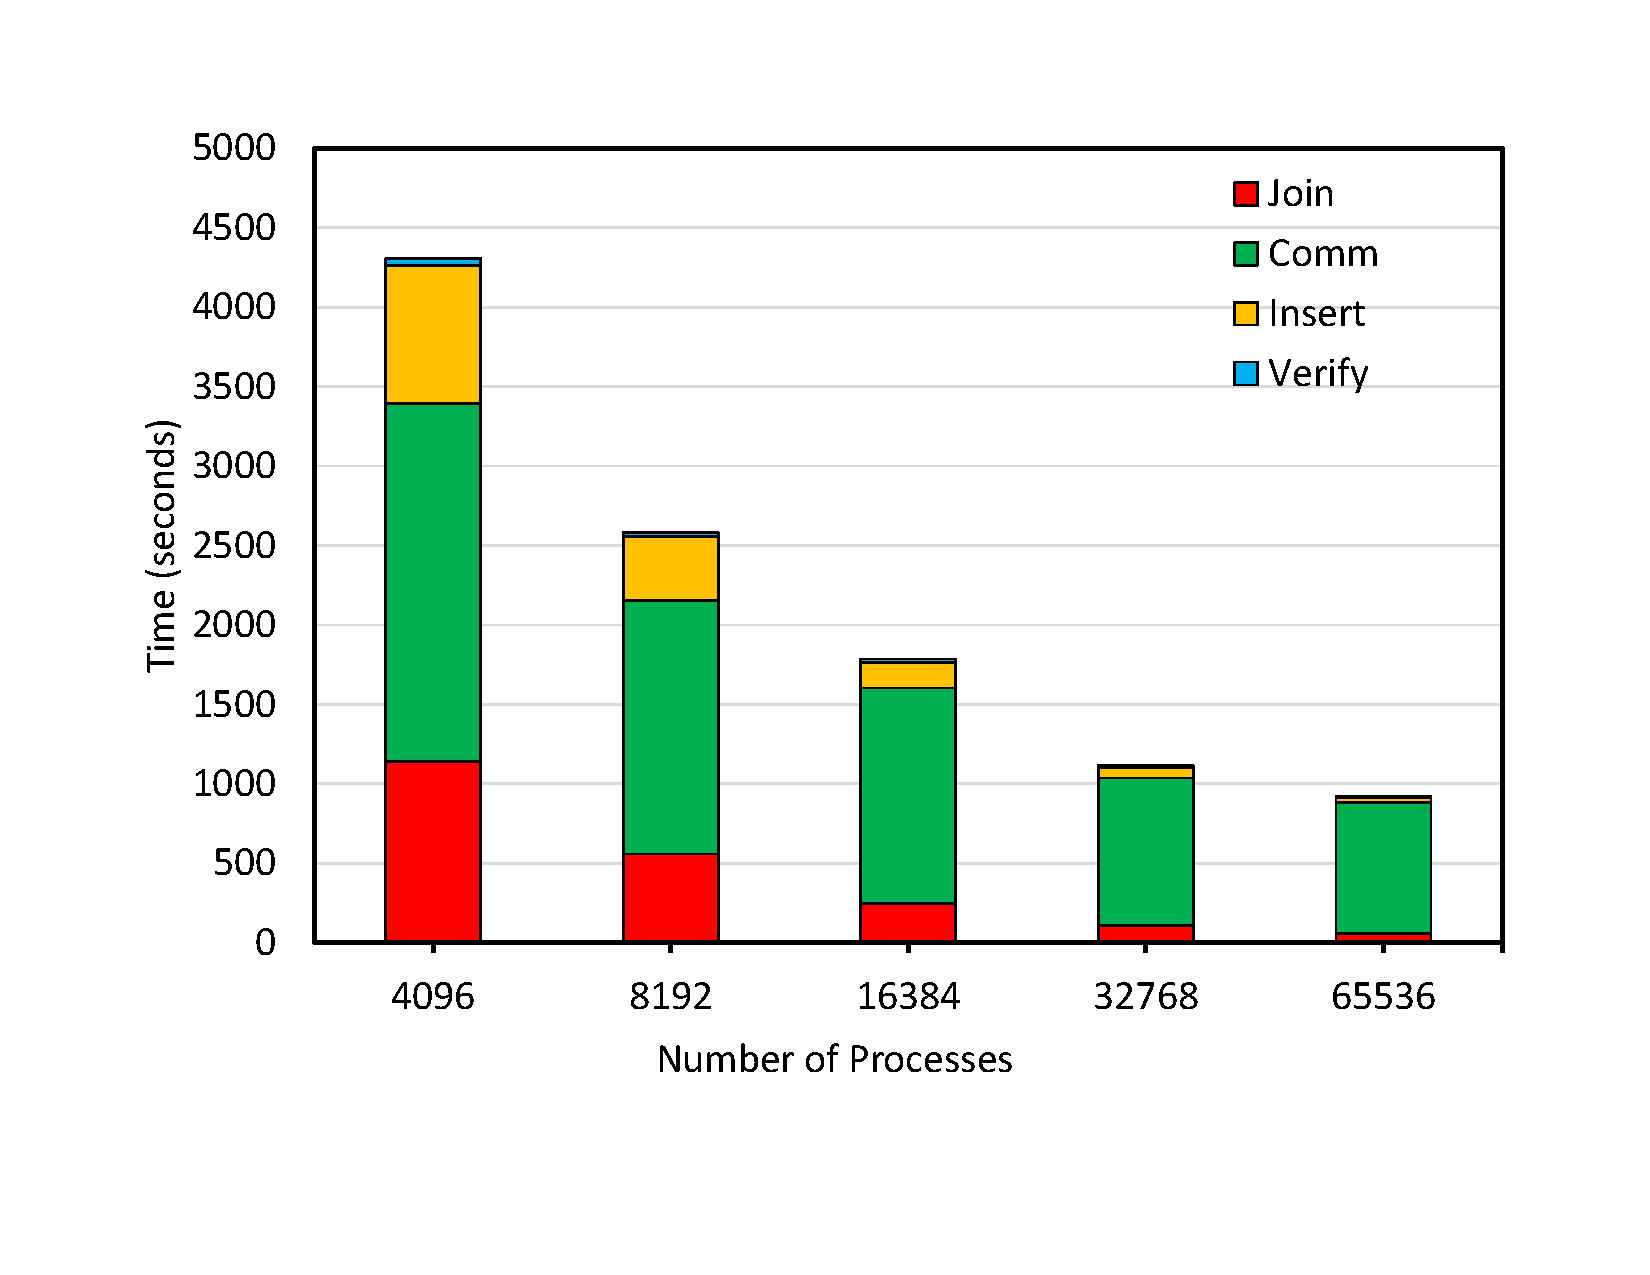
\includegraphics[width=.50\textwidth,  trim={0cm 0cm 0cm 0cm,
			clip}]{results/TC_260Billion_breakdown.pdf}}\hfill%
	\centering
	\caption{Transitive closure of a graph with X edges.}
	\label{fig:tc_large}
\end{figure*}